\chapter{Lecture 10 - MATLAB Built-in Methods and Error Estimates}
\label{ch:lec10n}
\section{Objectives}
The objectives of this lecture are to:
\begin{itemize}
\item Describe the most important MATLAB built-in method for finding the direct solution to linear systems of equations.
\item Define matrix norms and condition number.
\item Introduce an error estimate for solution of linear systems of equations.
\end{itemize}
\setcounter{lstannotation}{0}

\section{MATLAB Built-in Methods}
For most applications, the MATLAB function to use for solving linear systems of equations is \lstinline[style=myMatlab]{mldivide(A,b)} which is most conveniently accessed via the ``backslash'' operator \lstinline[style=myMatlab]{\}.

MATLAB's function \lstinline[style=myMatlab]{mldivide(A,b)} selects from an array of algorithms depending on the structure of \lstinline[style=myMatlab]{A}.  A portion of the logic is shown in Figure \ref{fig:lec10n-mldiv-part1}.
\marginnote[2.0cm]{Most algorithms require \lstinline[style=myMatlab]{A} to be square.  If \lstinline[style=myMatlab]{A} is not square, then \lstinline[style=myMatlab]{A} is not invertible and the problem is more aptly described as a least-squares linear fit that we will discuss in later lectures.  A ``QR solver'' carries out the decomposition \lstinline[style=myMatlab]{A=QR}, where \lstinline[style=myMatlab]{Q} is the same size as \lstinline[style=myMatlab]{A} but with orthonormal columns; \lstinline[style=myMatlab]{R} is $[n \times n]$ and upper triangular. 

\vspace{0.25cm}

\noindent If A is triangular or permuted triangular, back- or forward- substitution should be used instead of full Gauss elimination or LU factorization.}
\begin{figure}[h!]
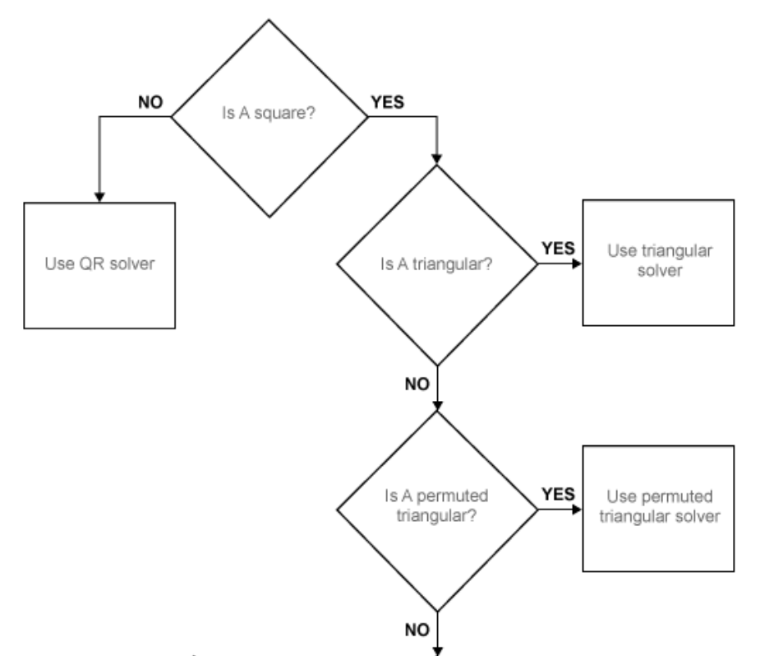
\includegraphics[width=0.6\textwidth]{lec10n_mldiv_part1.png}
\caption{Logic tree for \lstinline[style=myMatlab]{mldivide()}, part 1.}
\label{fig:lec10n-mldiv-part1}
\end{figure}


%\vspace{1.0cm}

\noindent The remaining logic tree for \lstinline[style=myMatlab]{mldivide(A,b)} is shown in Figure \ref{fig:lec10n-mldiv-part2}.
\marginnote[2.0cm]{A \emph{Hermitian} matrix satisfies the equality $A^{\star}=A$ where $A^{\star}$ denotes the transpose and complex conjugate of \lstinline[style=myMatlab]{A}.  Think of a Hermitian matrix as a symmetric matrix generalized for complex numbers.

\vspace{0.1cm}

\noindent If a matrix is Hermitian and if the matrix is positive definite (all positive or all negative entries along the diagonal being a hint that this property is true) then a Cholesky factorization is possible that is roughly twice as fast as an LU factorization.  Otherwise an LU factorization is used.

\vspace{0.1cm}

\noindent If \lstinline[style=myMatlab]{A} is not Hermitian, MATLAB checks if it, perchance, is upper Hessenberg. A matrix is \emph{upper Hessenberg} if it has non-zero entries on the upper triangular portion of \lstinline[style=myMatlab]{A} \emph{plus} is non-zero on the first diagonal below the main diagonal.  Matrices of this structure are formed as an intermediate step in matrix eigenvalue calculations.  A Hessenberg solver will take advantage of the zeros below the first sub-diagonal and find a solution more expeditiously than a general LU solver. 
}
\begin{figure}[h!]
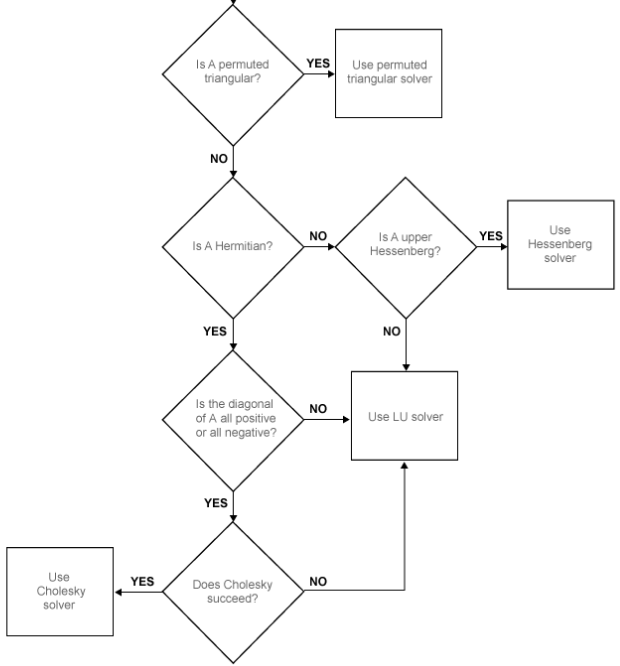
\includegraphics[width=0.6\textwidth]{lec10n_mldiv_part2.png}
\caption{Logic tree for \lstinline[style=myMatlab]{mldivide()}, part 2.}
\label{fig:lec10n-mldiv-part2}
\end{figure}

\newthought{As should be apparent}, a \emph{lot} of technology is crammed into the innocent-looking \lstinline[style=myMatlab]{mldivide} function.  We cannot hope to investigate all of these methods in this course.  I refer interested readers to an outstanding text by one of my favorite mathematical authors for a more thorough (and rigorous) overview of methods of numerical linear algebra.\cite{trefethen2022numerical}  Instead, I offer the following advice:
\begin{enumerate}
\item If the full matrix fits in memory and you only need to solve it once, use \lstinline[style=myMatlab]{mldivide(A,b)}---or just \lstinline[style=myMatlab]{'A\b'}.
\item Use a factorization, or \emph{decomposition}, if you must solve the system multiple times for different values of \lstinline[style=myMatlab]{b}. MATLAB offers a built-in function to do this: \lstinline[style=myMatlab]{decomposition{A,type)}, where the second (optional) argument is a string to specify the type of decomposition that is desired.  These types include: \lstinline[style=myMatlab]{'lu'}, \lstinline[style=myMatlab]{'qr'}, \lstinline[style=myMatlab]{'chol'}, and \lstinline[style=myMatlab]{'auto'} among others.\sidenote{When you select \lstinline[style=myMatlab]{type='auto'}, which also happens to be the default if no type is specified, MATLAB determines which decomposition is best.} 
An example listing using this feature is given below.
\begin{lstlisting}[style=myMatlab]
n = 5;
A = rand(n,n);
b1 = rand(n,1); b2 = rand(n,1);

Ad = decomposition(A,'auto');

x1 = Ad\b1;
x2 = Ad\b2;
\end{lstlisting}

\item If the matrix is very large, consider an iterative method that we will discuss in the next lecture.  In applications, large matrices tend to be \emph{sparse}---most of the elements are zero. The decomposition of large sparse matrices is often dense, however, so these methods may not be practical.  We will focus on this issue in the next lecture. 

\end{enumerate}

\section{Matrix Norms and Condition Number}
A norm is a real number assigned to a matrix or vector that satisfies the following four properties:
\begin{enumerate}
\item $||x||\ge 0$ and $||x||=0$ if and only  if $x = 0$.
\item $||\alpha x|| = \alpha ||x||$ for any constant $\alpha$.
\item $||Ax|| \le ||A||\ ||x||$ where $A$ is a matrix and $x$ is a vector of dimensions conformable with $A$.
\item For any two vectors $x$, and $y$: $||x + y|| \le ||x|| + ||y||$.  This is referred to as the ``triangle inequality.''  
\end{enumerate}
Some common vector and matrix norms are defined in Table \ref{tab:matrix-and-vector-norms}.
\begin{table}
\begin{tabular}{| c | c |}
\hline
Vector Norms & Matrix Norms \\ \hline
\multirow{2}{*}{$||x||_{\infty} = \max\limits_{1 \le i \le n} |x_i|$} &  $||A||_{\infty} = \max\limits_{1 \le i \le n} \sum\limits_{j=1}^{n} |a_{ij}|  $ \\ 
  & max sum of row absolute value \\ \hline
\multirow{2}{*}{$||x||_{1} = \sum\limits_{i=1}^{n} |x_{i}|$} & $||A||_1 = \max\limits_{1\le j \le n}\sum\limits_{i=1}^{n} |a_{ij}|$ \\ 
 & max sum of column absolute value \\ \hline
 \multirow{2}{*}{$||x||_2 = \left(\sum\limits_{i=1}^{n} |x_{i}|^2 \right)^{\sfrac{1}{2}}   $} & $||A||_2 = \max\left(\frac{||Ax||_2}{||x||_2}\right) $\\
 &  over all vectors $x$ \\ \hline
\end{tabular}
\caption{Common vector and matrix norms.}
\label{tab:matrix-and-vector-norms}
\end{table}
\marginnote[-3.0cm]{A generalization of the vector norms presented is the $p$-norm:
$$||x||_{p} = \left(\sum\limits_{i=1}^{n} |x_i|^{p} \right)^{\sfrac{1}{p}}$$
As $p$ increases, the value of $\max\limits_{1 \le i \le n}|x_{i}|^p$ gets large relative to all of the other values of $|x_i|^p$; in the limit of $p\to \infty$ only the largest value $|x_i|^p$ matters and thus we get the ``infinity norm'': $||x||_{\infty}$.  

\vspace{0.1cm}

\noindent A less common matrix norm is the Frobenius norm or ``taxi-cab'' norm:
$$||A||_{F} = \left(\sum\limits_{i=1}^{m} \sum\limits_{j=1}^{n} |a_{ij}|^2 \right)^{\sfrac{1}{2}}$$
which, if nothing else, has a fun name.
}
The matrix 2-norm---$||A||_{2}$---is \emph{induced} from the vector 2-norm.  It is meant to characterize the \emph{action} of the matrix $A$ on some vector $x$.  For this book, the most important norm is the vector 2-norm and the induced matrix 2-norm.  If the type of norm is not mentioned, you should assume it is a 2-norm.

\subsection{Matrix Condition Number}
The condition number is a useful property of a matrix.  It is defined by Equation \ref{eq:lec10n-matrix-condition}:
\begin{equation}
\kappa(A) = ||A|| \ ||A^{-1}||
\label{eq:lec10n-matrix-condition}
\end{equation}
where $|| \cdot ||$ refers to any valid matrix norm.  Some important condition number facts\sidenote{If you find this to be boring, Google ``Chuck Norris Facts'' instead. } include:
\begin{enumerate}
\item The condition number of the identity matrix (of any size) is 1.
\item All other matrices have a condition number of 1 or greater.
\item The numerical value of $\kappa(A)$ depends on the norm used in calculating it but, generally speaking, a matrix that has a very large condition number is said to be \emph{ill conditioned}.
\item In the matrix 2-norm, the matrix condition number is equal to:\marginnote{The singular value decomposition (SVD) of a matrix $A$ is given by:
$$A = U\Sigma V^{*}  $$
where $U$ and $V^{*}$ are orthonormal matrices in which the columns are referred to as left singular vectors and right singular vectors respectively and $\Sigma$ is a diagonal matrix with the singular values of $A$.  The SVD of a real symmetric matrix is related to the eigenvalue decomposition:
$$A^{*}A = V\Sigma^{*}\Sigma V^{*}  $$
where $\Sigma$ is a diagonal matrix with the eigenvalues along the diagonal.
} 
$$\kappa(A) = \frac{\sigma_{\text{max}}}{\sigma_{\text{min}}}$$
where $\sigma$ are singular values.  For real, symmetric matrices, the singular values are equal to the absolute values of the eigenvalues.
\end{enumerate}

\section{Relative Error Bounds}
We can use the condition number of a matrix to derive error bounds on the solution to a linear system of equations.  As a reminder, for a numeric solution to a linear system of equations, we can define the residual as:
\begin{equation*}
r = Ax^{NS}-b
\end{equation*}
where $x^{NS}$ is the numeric solution.  The relative residual is:
\begin{equation*}
\text{relative residual } = \frac{||r||}{||b||}
\end{equation*}
Also recall that we define the error as:
\begin{equation*}
e = x^{\star} - x^{NS}
\end{equation*}
where $x^{\star}$ is the exact solution. The relative error is:
\begin{equation*}
\text{relative error } = \frac{||e||}{||x^{\star}||}
\end{equation*}
We would like to know what the relative error is but, in general, we do not know the exact solution.  What we \emph{can} do is obtain a bound on the relative error based on the condition number and relative residual; both of which we can compute.  This error bound is given in Equation \ref{eq:lec10n-error-bound}.
\begin{equation}
\frac{1}{\kappa(A)}\frac{||r||}{||b||} \le \frac{||e||}{||x^{\star}||} \le \kappa(A) \frac{||r||}{||b||}
\label{eq:lec10n-error-bound}
\end{equation}
We can use this expression to predict an error bound and quantify the impact of attempting to solve an ill conditioned system of equations.

